\documentclass[10pt]{beamer}

\usepackage{fontspec}
\setmainfont{Ubuntu}[]
\setsansfont{Ubuntu}[]
\setmonofont{Ubuntu Mono}[]

\usepackage{graphicx}
\graphicspath{ {../../lesson_13/img/} }

\beamertemplatenavigationsymbolsempty

\title{Свойства BEAM}

\begin{document}

\begin{frame}
  \centering
  Эликсир и Эрланг объединяет виртуальная машина
  \textbf{Erlang~Virtual~Machine}
  \par \bigskip
  которую обычно называют \textbf{BEAM}
  (Bogdan's~Erlang~Abstract~Machine).
\end{frame}

\begin{frame}
    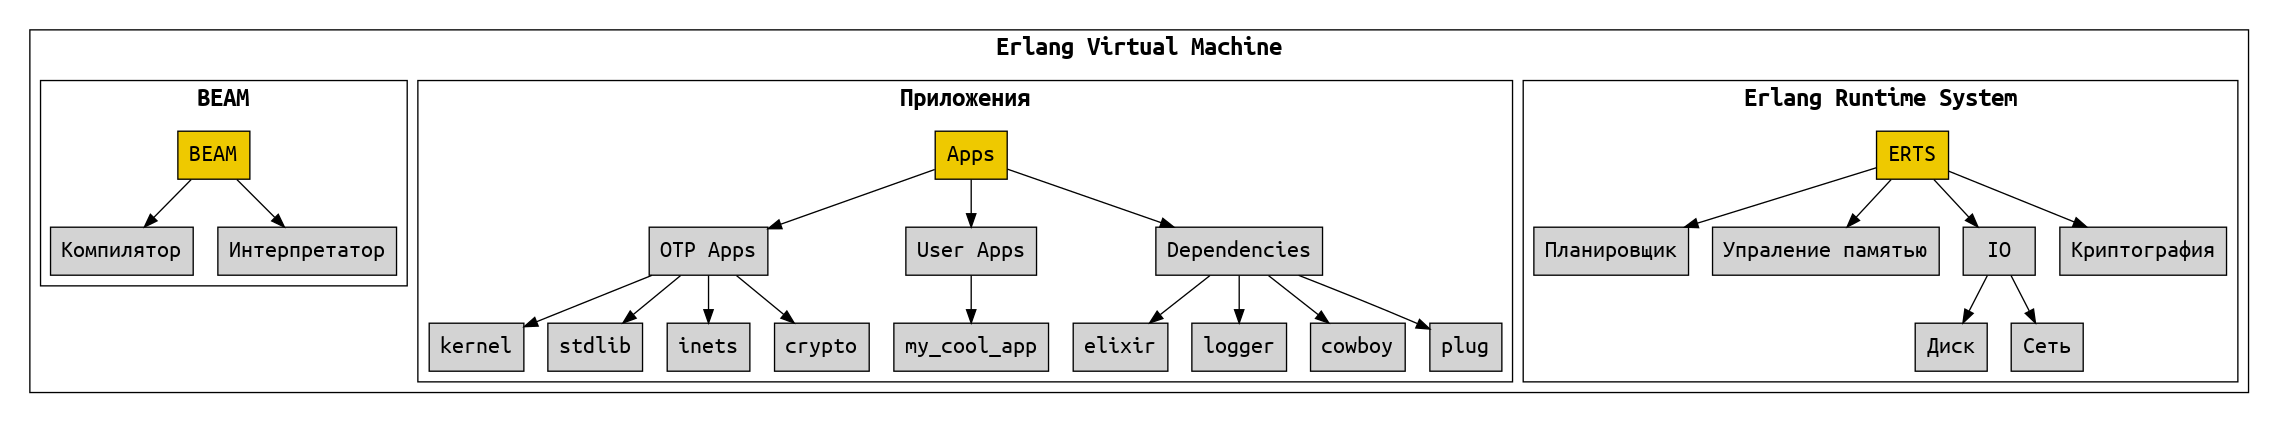
\includegraphics[scale=0.2]{release}
\end{frame}

\end{document}
